\chapter{Linfomi}

\section{Introduzione ai linfomi}
I linfomi sono tumori causati dalla proliferazione incontrollata dei linfociti.
All’interno del linfocita si ha la comparsa di mutazioni che coinvolgono un numero elevato di geni, 
implicati nella proliferazione, crescita e morte dei linfociti stessi.
I linfociti mutati vanno a invadere principalmente i linfonodi, creando degli accumuli patologici al loro interno, 
ma tale patologia può coinvolgere tutti gli organi.  
I linfomi si presentano con caratteristiche estremamente variabili, in virtù del fatto che le mutazioni 
possono insorgere in diverse fasi dello sviluppo del linfocita\cite{LINFOMIAIL}.\\

In base all’origine cellulare, si distinguono i linfomi che originano dalla linea T, 
più rari nelle popolazioni occidentali, e i linfomi che originano dalla linea B che sono i più frequenti. 
Distinguiamo i linfomi di Hodgkin, che originano dalla trasformazione dei linfociti B; 
i linfomi non-Hodgkin in cui sono coinvolte entrambe le tipologie di linfociti, sia B che T.\\

Le cause e i fattori di rischio che possono dare origine a tale malattia, sono in gran parte sconosciuti, 
è noto che infezioni causate da alcuni virus e batteri, così come alcune malattie croniche, 
si possono ritenere responsabili dell’aumento del rischio dello sviluppo di alcuni sottotipi di linfoma\cite{LINFOMIAIL}.\\

\section{Linfoma non-Hodgkin}

\begin{figure}[h]
    \begin{center}
    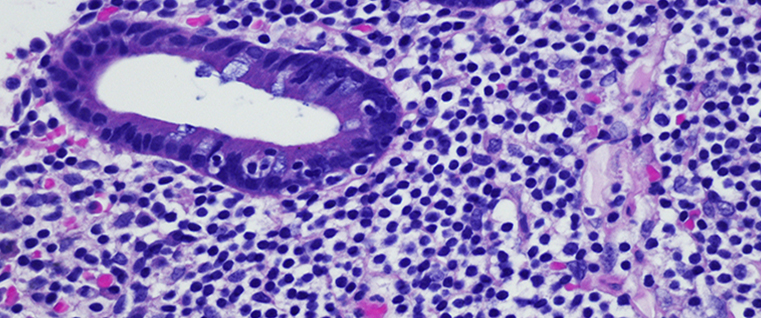
\includegraphics[width=0.6\columnwidth]{img/Linfoma-non-Hodgkin.jpeg}
    \end{center}
    \caption[Aspetto del linfoma non-hodgkin al microscopio]{Aspetto del linfoma non-hodgkin al microscopio
    \cite{img3}}

\end{figure}

I linfomi non-Hodgkin (LNH) sono neoplasie che originano dalla proliferazione incontrollata dei linfociti B e T; 
tali cellule fanno parte del sistema immunitario e si trovano nel sangue, nel tessuto linfatico di linfonodi, milza, 
timo e midollo osseo\cite{LNHAIL}.\\ 
Nel LNH i linfociti creano accumuli patologici all’interno dei linfonodi. La differenza tra i LNH e il 
linfoma di Hodgkin è l’assenza della cellula di Reed-Sternberg, un particolare tipo di linfocita B caratterizzato 
dalla presenza di due nuclei, che permette di distinguere una cellula sana da una malata\cite{LNHAIMAC}.\\

\section{Cause}
Ad oggi non sono chiare le cause che portano alla comparsa di tale patologia, sappiamo che è la mutazione del 
DNA del linfocita che porta allo sviluppo di tale neoplasia, ma non sono ancora note le cause per cui tale 
mutazione si verifica.\\ 
Tuttavia, alcuni fattori aumentano il rischio di sviluppo di determinati sottotipi di linfoma come ad esempio 
l’immunodepressione, quindi l’ indebolimento del sistema immunitario, causato ad esempio da terapie con farmaci 
immunosoppressori usati nel post-trapianto o in caso di infezione da HIV, che indebolisce anch’esso 
il sistema immunitario.\\ 

Ma anche malattie autoimmuni, come il Lupus eritematoso sistemico (LES), artrite reumatoide, 
la malattia di Sjogren (Sjögren), la celiachia sono correlate ad un aumento del rischio di sviluppo del NHL, 
in quanto l’iperattività del sistema immunitario in questo tipo di malattie può provocare la crescita e la 
divisione dei linfociti in modo incontrollato, 
e ciò può comportare lo sviluppo di cellule anomale\cite{AMERICANCS}.\\

Sono fonte di rischio anche le infezioni virali croniche, in quanto il sistema immunitario, 
per combattere l’infezione, stimola una maggiore produzione di linfociti, che può aumentare il rischio che si 
verifichino mutazioni nel DNA del linfocita stesso. Esempi di infezioni virali croniche sono l’epatite C, 
la precedente esposizione al virus di Epstein-Barr (responsabile della mononucleosi infettiva), 
l'infezione da virus della leucemia umana a cellule T (HTLV-1), maggiormente diffuso in alcune parti del 
Giappone e nei Caraibi, ma si può trovare in tutto il mondo (la trasmissione è sessuale, mediante sangue infetto 
oppure tramite il latte materno da una madre infetta); l’infezione da virus dell'herpes umano 8 (HHV-8), 
può causare un linfoma molto raro, noto come linfoma a versamento primario, che si presenta in soggetti infetti da HIV.\\

Le infezioni batteriche, rappresentano anch’esse un fattore di rischio nello sviluppo del LNH. 
L’infezione causata da Helicobacter pylori, rappresenta la prima causa di linfoma primitivo dello stomaco; 
la Chlamydophila psittaci, è un batterio collegato allo sviluppo del linfoma nei tessuti intorno all’occhio, 
chiamato linfoma della zona marginale annessiale oculare; il batterio Campylobacter jejuni è correlato a un tipo 
di linfoma MALT, chiamato malattia immunoproliferativa dell'intestino tenue\cite{AMERICANCS}.\\
Inoltre, il trattamento con chemioterapia o radioterapia, a cui è sottoposta la persona a causa di altri tipi di tumore, 
può aumentare negli anni seguenti  il rischio di sviluppare il LNH\cite{AMERICANCS}.\\

L’esposizione a sostanze chimiche tossiche, come pesticidi e derivati del benzene, è un fattore di rischio. 
Il linfoma non Hodgkin non sembra essere presente in più membri di una stessa famiglia, tuttavia, 
il rischio può essere leggermente maggiore se un parente di primo grado (come un genitore o un fratello/sorella) 
ha avuto il linfoma\cite{AMERICANCS}.\\
Il linfoma può colpire a qualunque età, però c’è un maggiore rischio nella sesta decade di vita, 
maggiormente negli uomini piuttosto che nelle donne, ma alcuni sottotipi di LNH si manifestano 
maggiormente nelle donne, per cause non ancora note. 
Un maggiore rischio si presenta inoltre nei paesi industrializzati e nella razza bianca\cite{AMERICANCS}.\\ 

\section{Epidemiologia}
I linfomi non Hodgkin rappresentano globalmente il 4-5\% delle nuove diagnosi di neoplasia nella popolazione 
occidentale e in Italia 
sono la quinta forma di cancro più comune negli uomini e la sesta nelle donne\cite{AIOM}. 
L’età media di insorgenza è compresa tra i 50 e 60 anni e l’incidenza tende a incrementare con l’aumentare dell’età. 
Il LNH può tuttavia presentarsi ad ogni età.\\ 
In Italia si calcolano circa 19-20 nuovi casi per 100.000 abitanti ogni anno, pertanto 16.000 nuovi casi di linfoma, 
con un incremento annuo pari all’1,3\%\cite{AIOM}.\\
L’incidenza dei linfomi risulta essere influenzata da fattori geografici, razziali e dall'età, 
pertanto avremo una maggiore incidenza nei paesi industrializzati, negli uomini e nella razza bianca\cite{AIOM}.\\
L’incidenza è in aumento, secondo le stime dei Registri Tumori AIRTUM. “L’Associazione Italiana Registri Tumori 
(AIRTUM) nasce a Firenze nel 1996 con lo scopo di promuovere, coordinare e sostenere l’attività di registrazione 
dei tumori in Italia\cite{AIRTUM}.”\\
Per l’anno 2020 le stime parlano circa di 7000 nuovi casi tra gli uomini e 6100 tra le donne come raffigurato 
in Figura \ref*{fig:FIGURE_2.2}. 
Nonostante ciò, la mortalità resta stabile negli anni\cite{AIRC}.\\
In America, il LNH è uno dei tumori più diffusi, rappresenta circa il 4\% delle diagnosi di tumore. 
Secondo le stime dell’American Cancer Society, negli Stati Uniti nel 2022 sono previste circa 80.000 nuove 
diagnosi di LNH e circa 20.000 decessi\cite{Americanstatistic}.\\

\begin{figure}[H]
    \begin{center}
    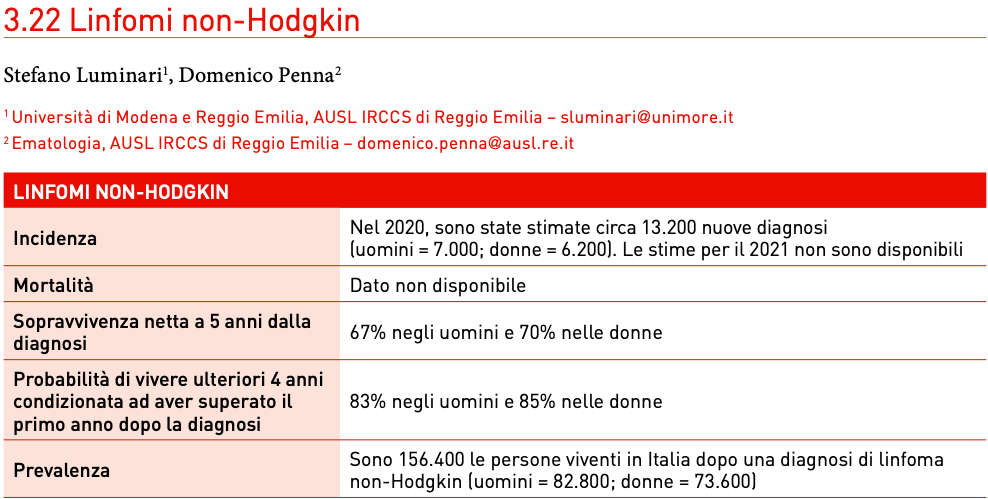
\includegraphics[width=0.8\columnwidth]{img/2021.png}
    \end{center}
    \caption{Numeri del cancro in Italia per l’anno 2021
    \cite{img4}}
    \label{fig:FIGURE_2.2}
\end{figure}

\begin{figure}[H]
    \begin{center}
    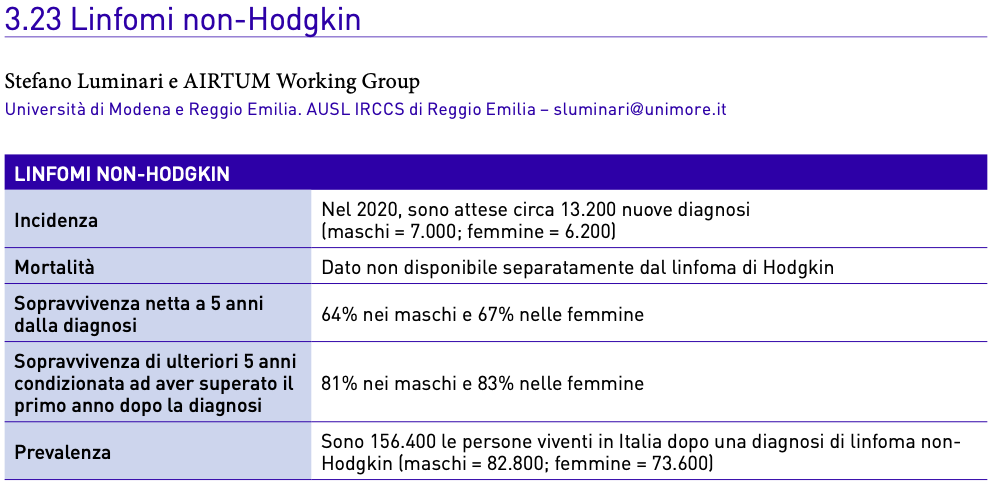
\includegraphics[width=0.8\columnwidth]{img/2020.png}
    \end{center}
    \caption[Numeri del cancro in Italia per l’anno 2020]{Numeri del cancro in Italia per l’anno 2020
    \cite{img5}}

\end{figure}

\begin{figure}[H]
    \begin{center}
    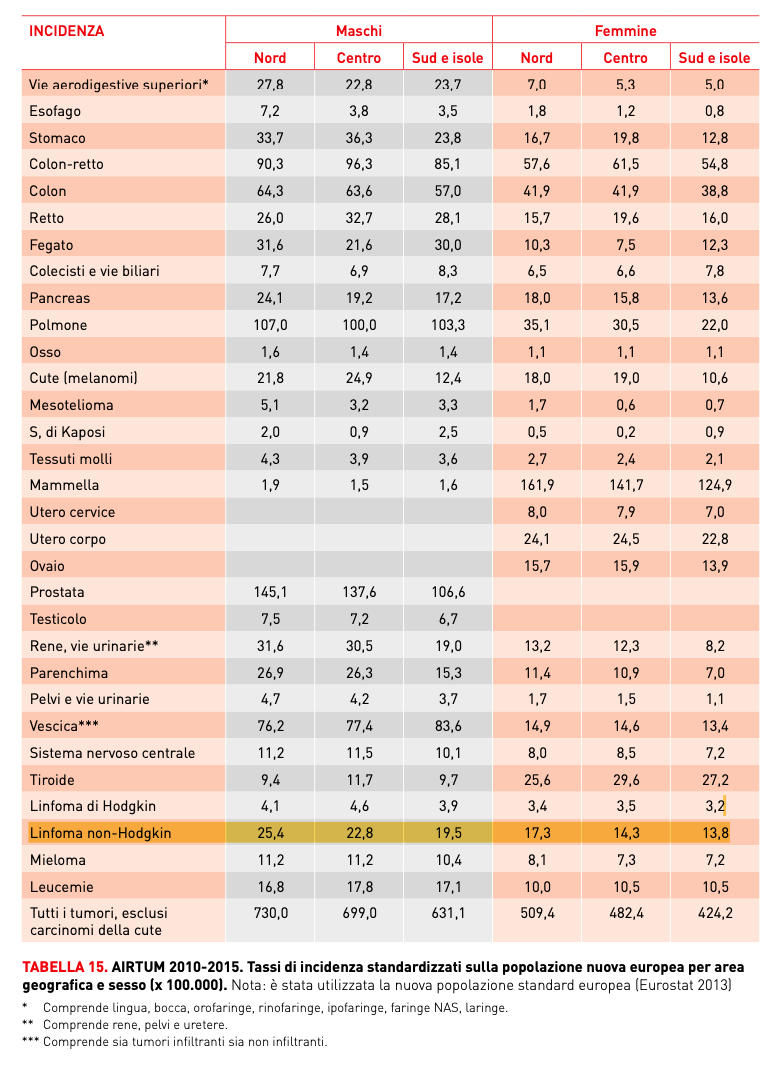
\includegraphics[width=0.8\columnwidth]{img/INCIDENZA.png}
    \end{center}
    \caption[Registro tumori AIRTUM. Tasso di incidenza anni 2010-2015.]{Registro tumori AIRTUM. Tasso di incidenza anni 2010-2015.
    \cite{img6}}

\end{figure}

\begin{figure}[H]
    \begin{center}
    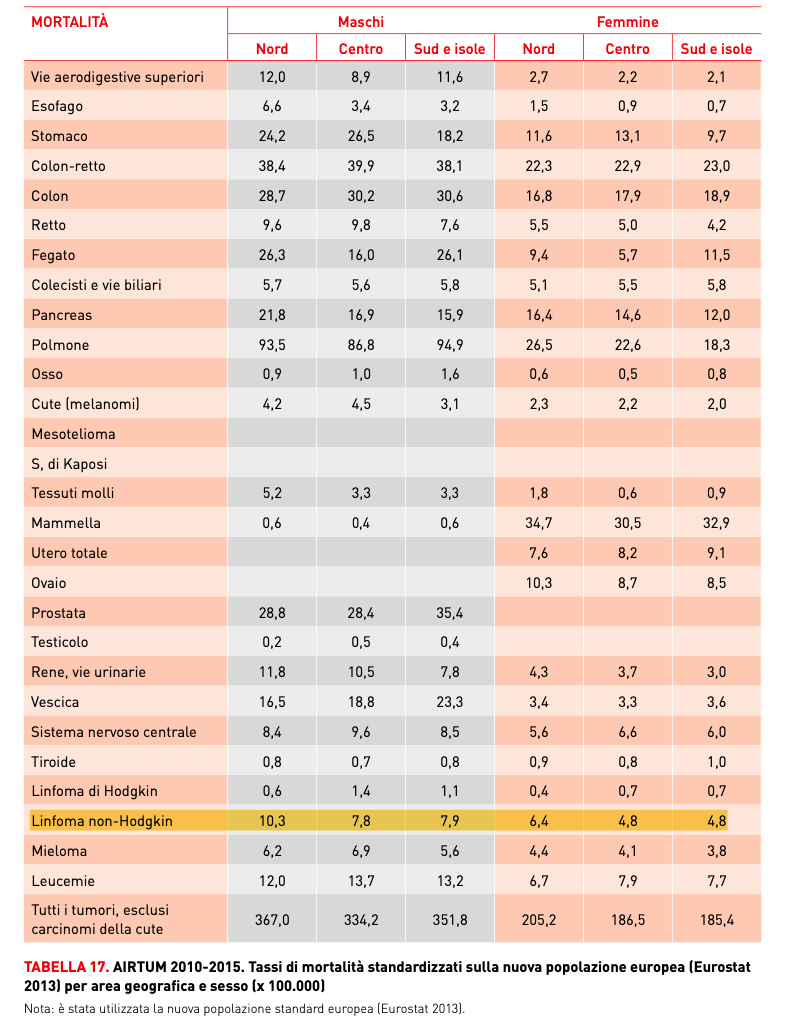
\includegraphics[width=0.8\columnwidth]{img/MORTALITA.png}
    \end{center}
    \caption[Registro tumori AIRTUM. Tasso di mortalità anni 2010-2015.]{Registro tumori AIRTUM. Tasso di mortalità anni 2010-2015.
    \cite{img7}}

\end{figure}

\begin{figure}[H]
    \begin{center}
    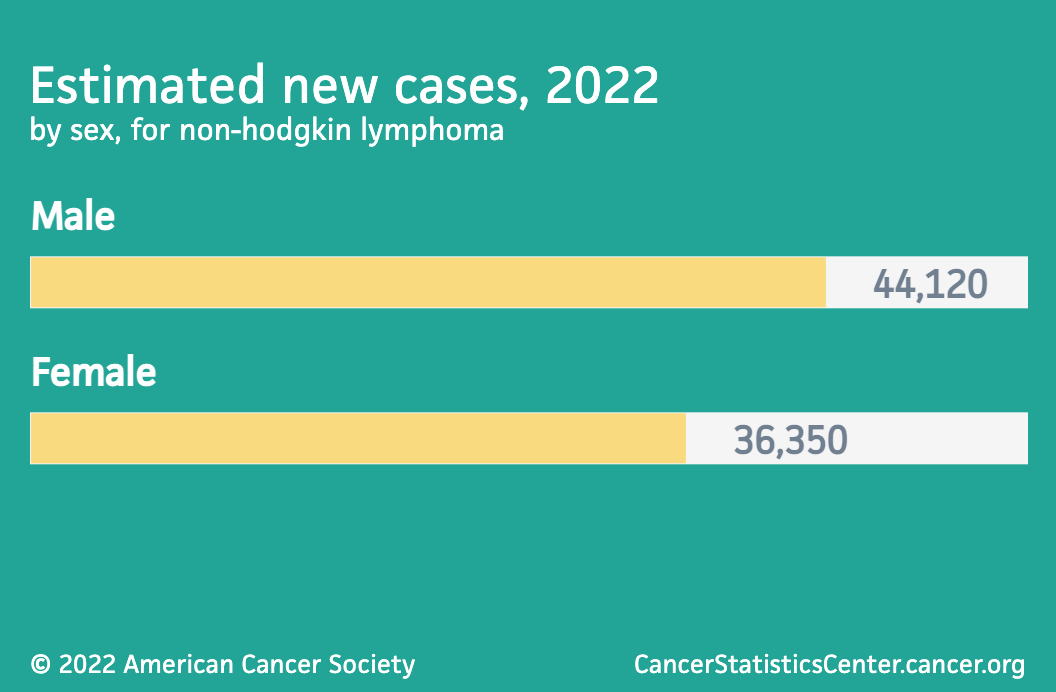
\includegraphics[width=0.5\columnwidth]{img/Estimatednewcases2022.png}
    \end{center}
    \caption[Stime dei nuovi casi di LNH negli Stati Uniti per l’anno 2022.]{Stime dei nuovi casi di LNH negli Stati Uniti per l’anno 2022.
    \cite{img8}}

\end{figure}

\begin{figure}[H]
    \begin{center}
    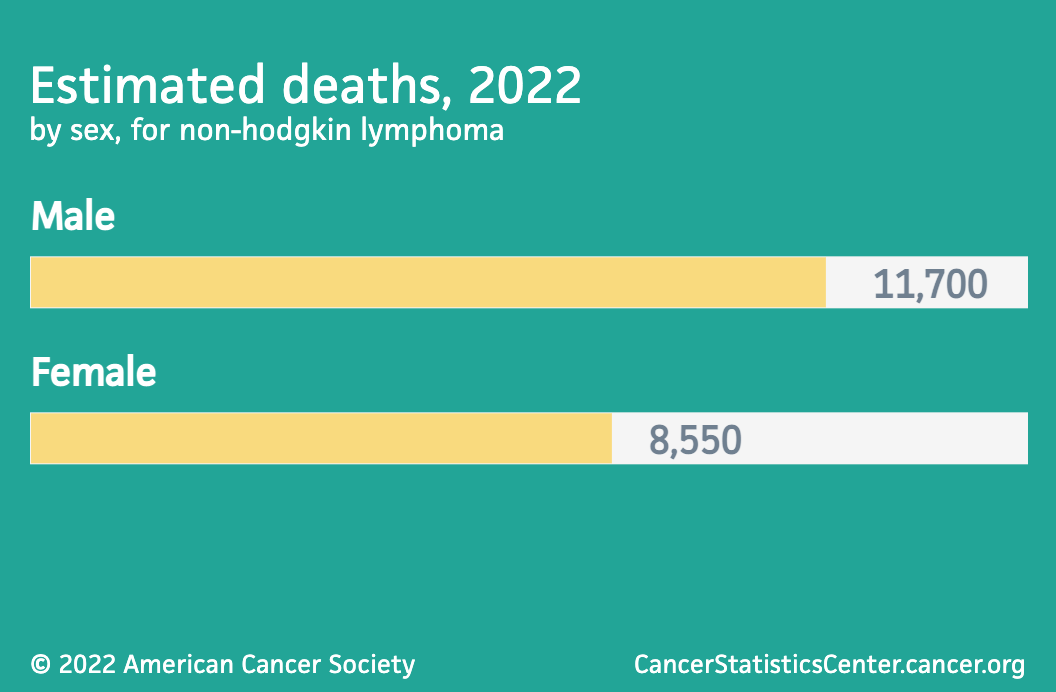
\includegraphics[width=0.5\columnwidth]{img/Estimateddeaths2022.png}
    \end{center}
    \caption[Stime decessi LNH negli Stati Uniti per l’anno 2022.]{Stime decessi LNH negli Stati Uniti per l’anno 2022.
    \cite{img9}}

\end{figure}

\begin{figure}[H]
    \begin{center}
    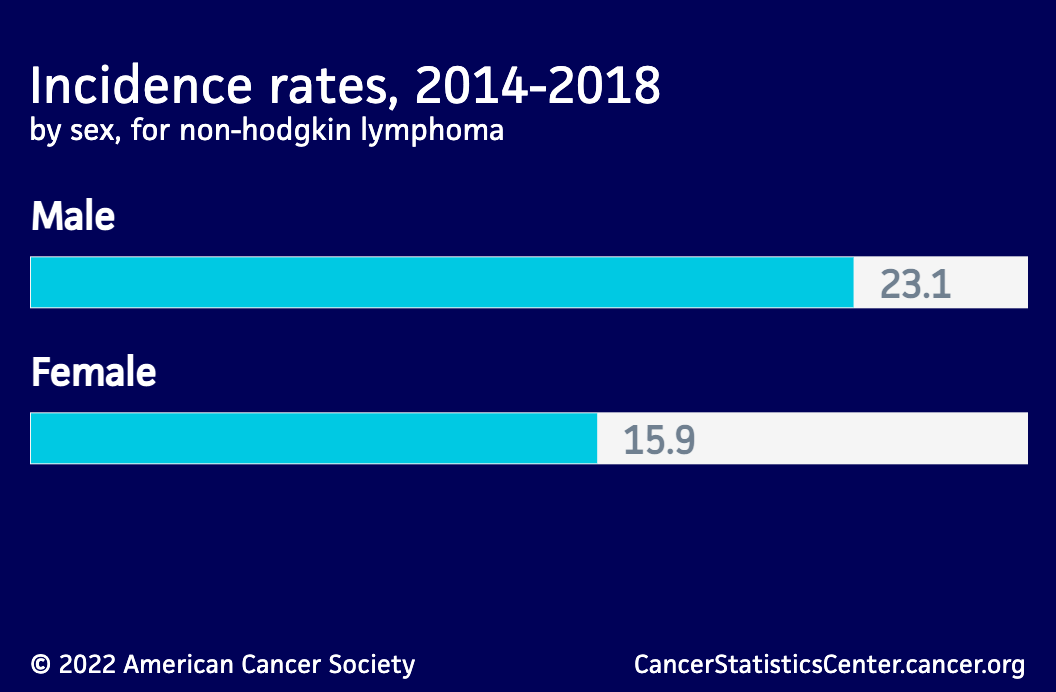
\includegraphics[width=0.5\columnwidth]{img/Incidencerates2014-18.png}
    \end{center}
    \caption[Tassi di incidenza del LNH negli anni 2014-2018 negli Stati Uniti.]{Tassi di incidenza del LNH negli anni 2014-2018 negli Stati Uniti.
    \cite{img10}}

\end{figure}

\begin{figure}[H]
    \begin{center}
    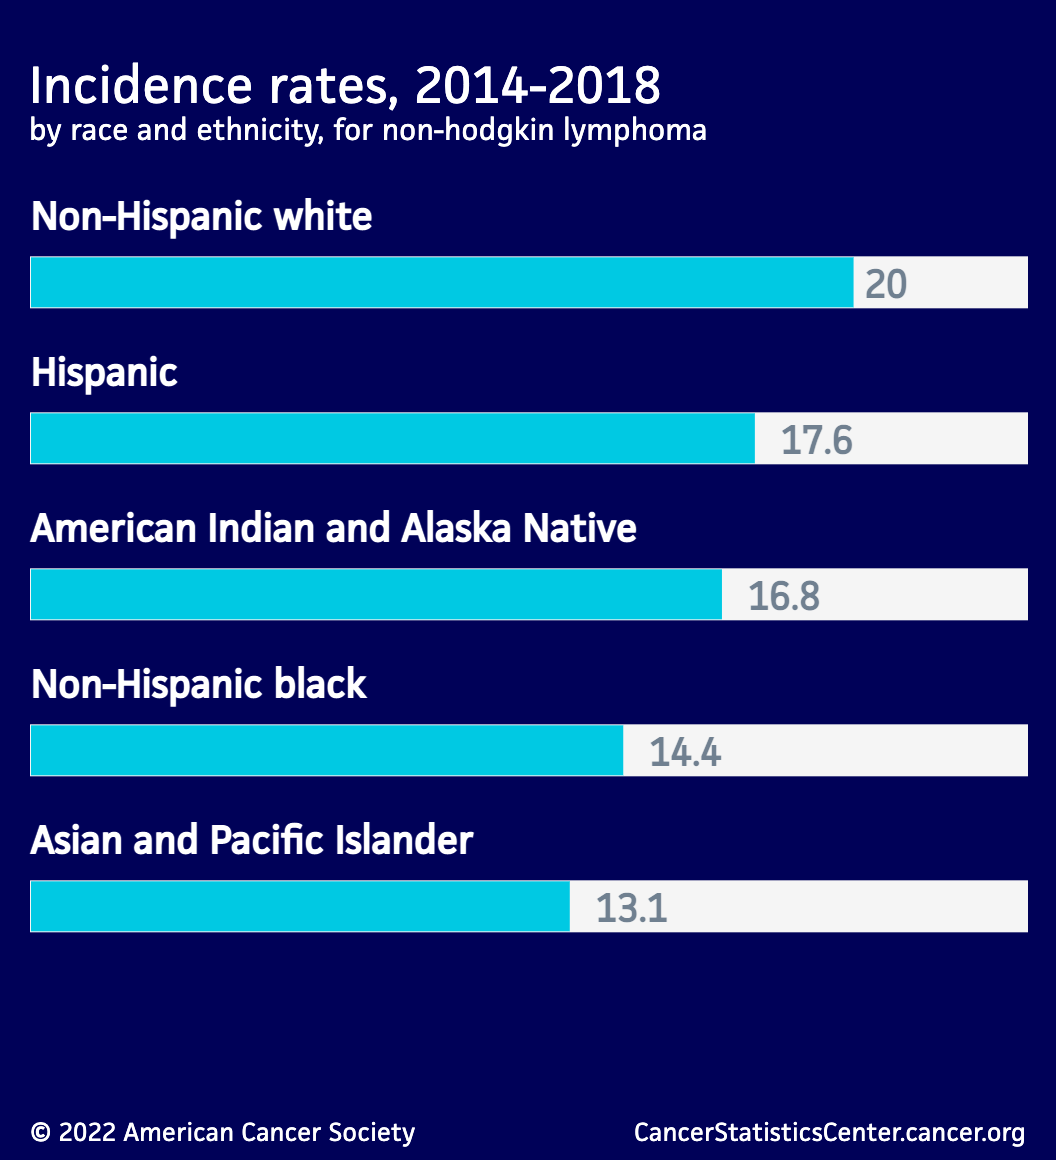
\includegraphics[width=0.4\columnwidth]{img/Incidencerates2014-18race-ethnicity.png}
    \end{center}
    \caption[Tassi di incidenza del LNH divisi per etnia, negli anni 2014-2018 negli Stati Uniti.]{Tassi di incidenza del LNH divisi per etnia, negli anni 2014-2018 negli Stati Uniti.
    \cite{img11}}

\end{figure}

\begin{figure}[H]
    \begin{center}
    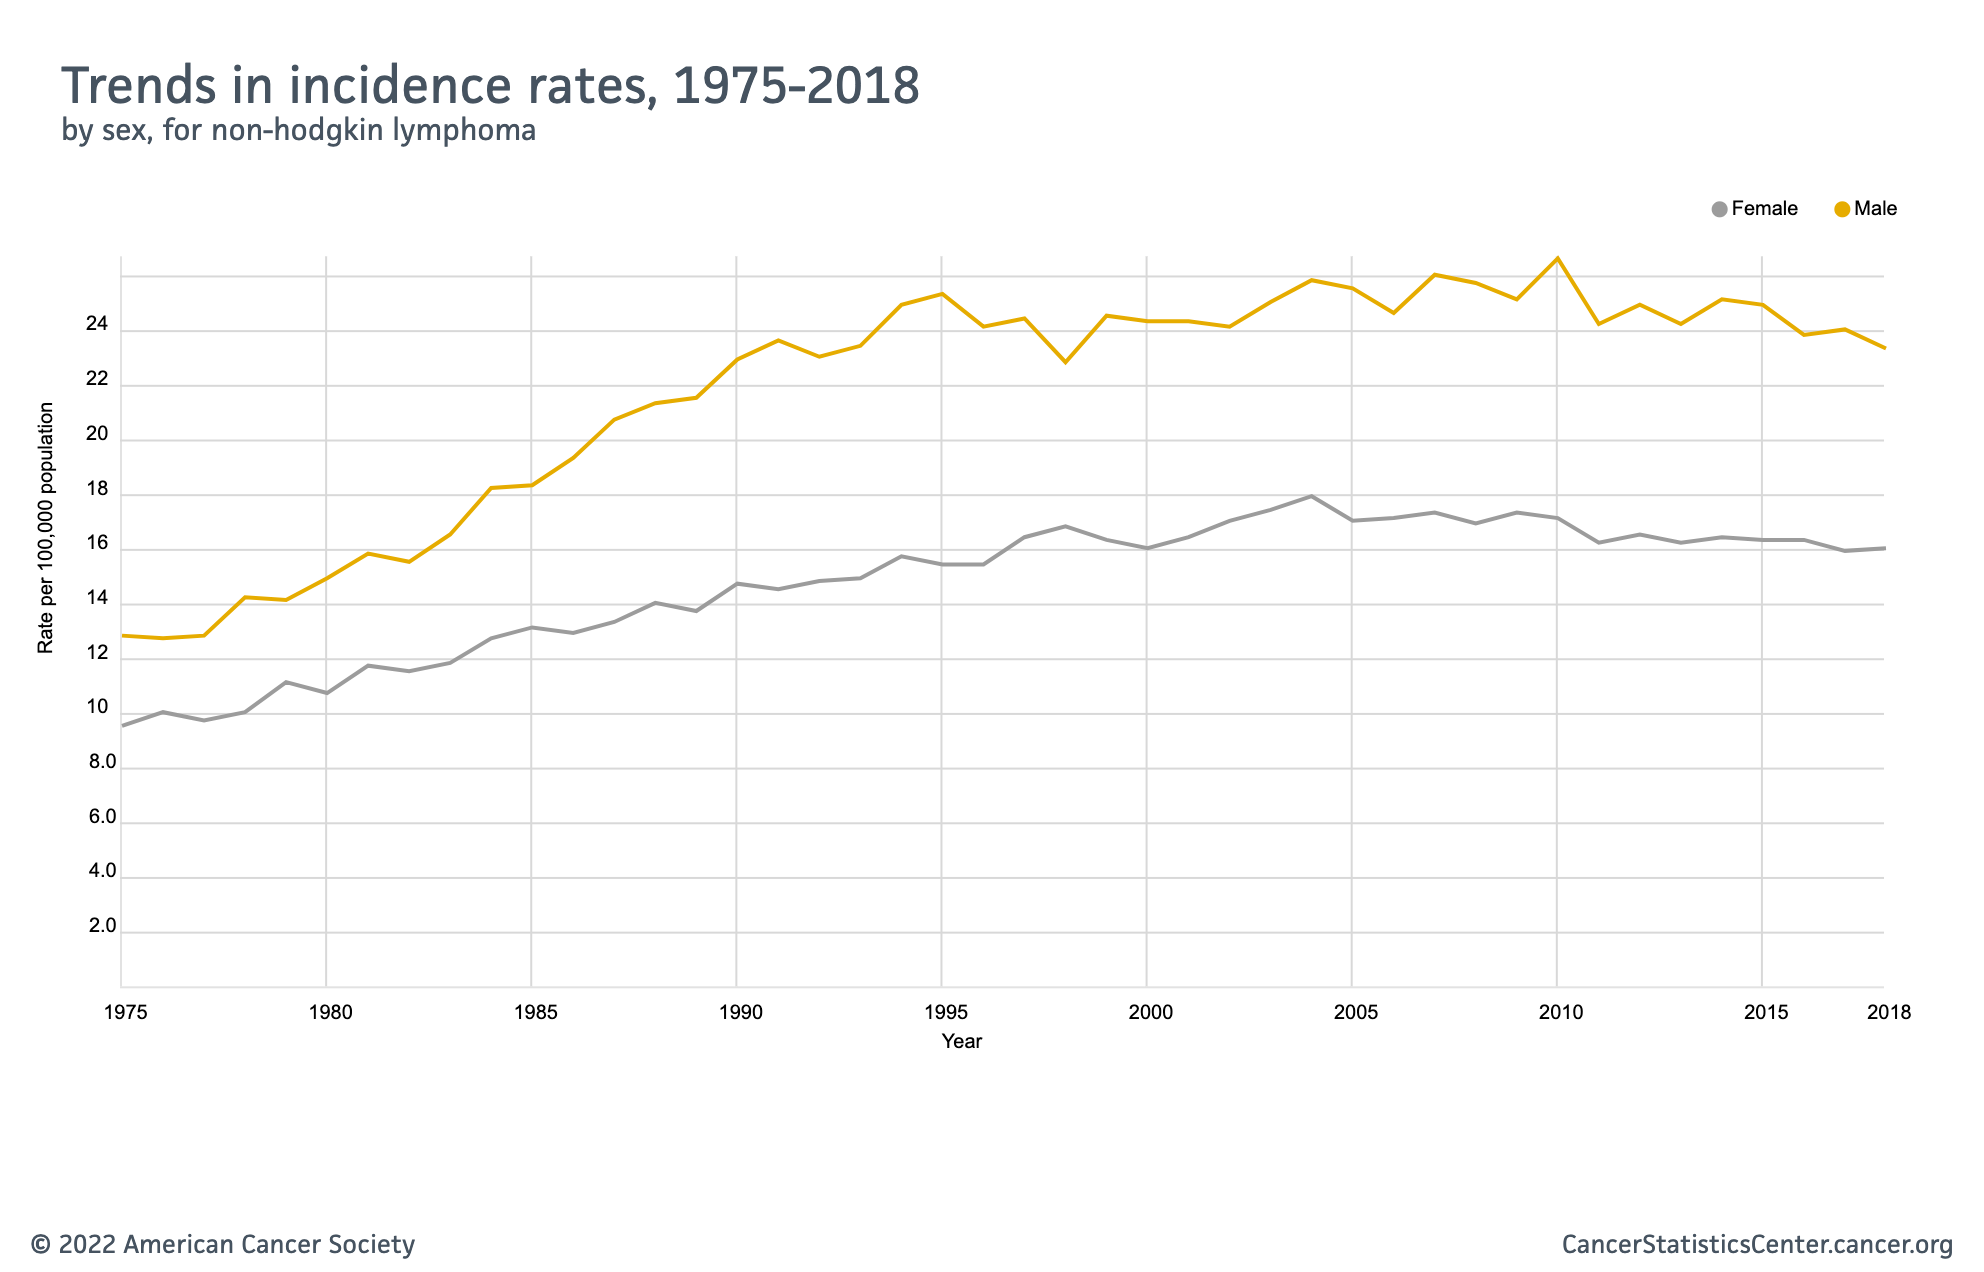
\includegraphics[width=0.8\columnwidth]{img/Incidencerates1975-2018.png}
    \end{center}
    \caption[Tassi di incidenza del LNH in base al sesso, anni 1975-2018 negli Stati Uniti.]{Tassi di incidenza del LNH in base al sesso, anni 1975-2018 negli Stati Uniti.
    \cite{img12}}

\end{figure}

\begin{figure}[H]
    \begin{center}
    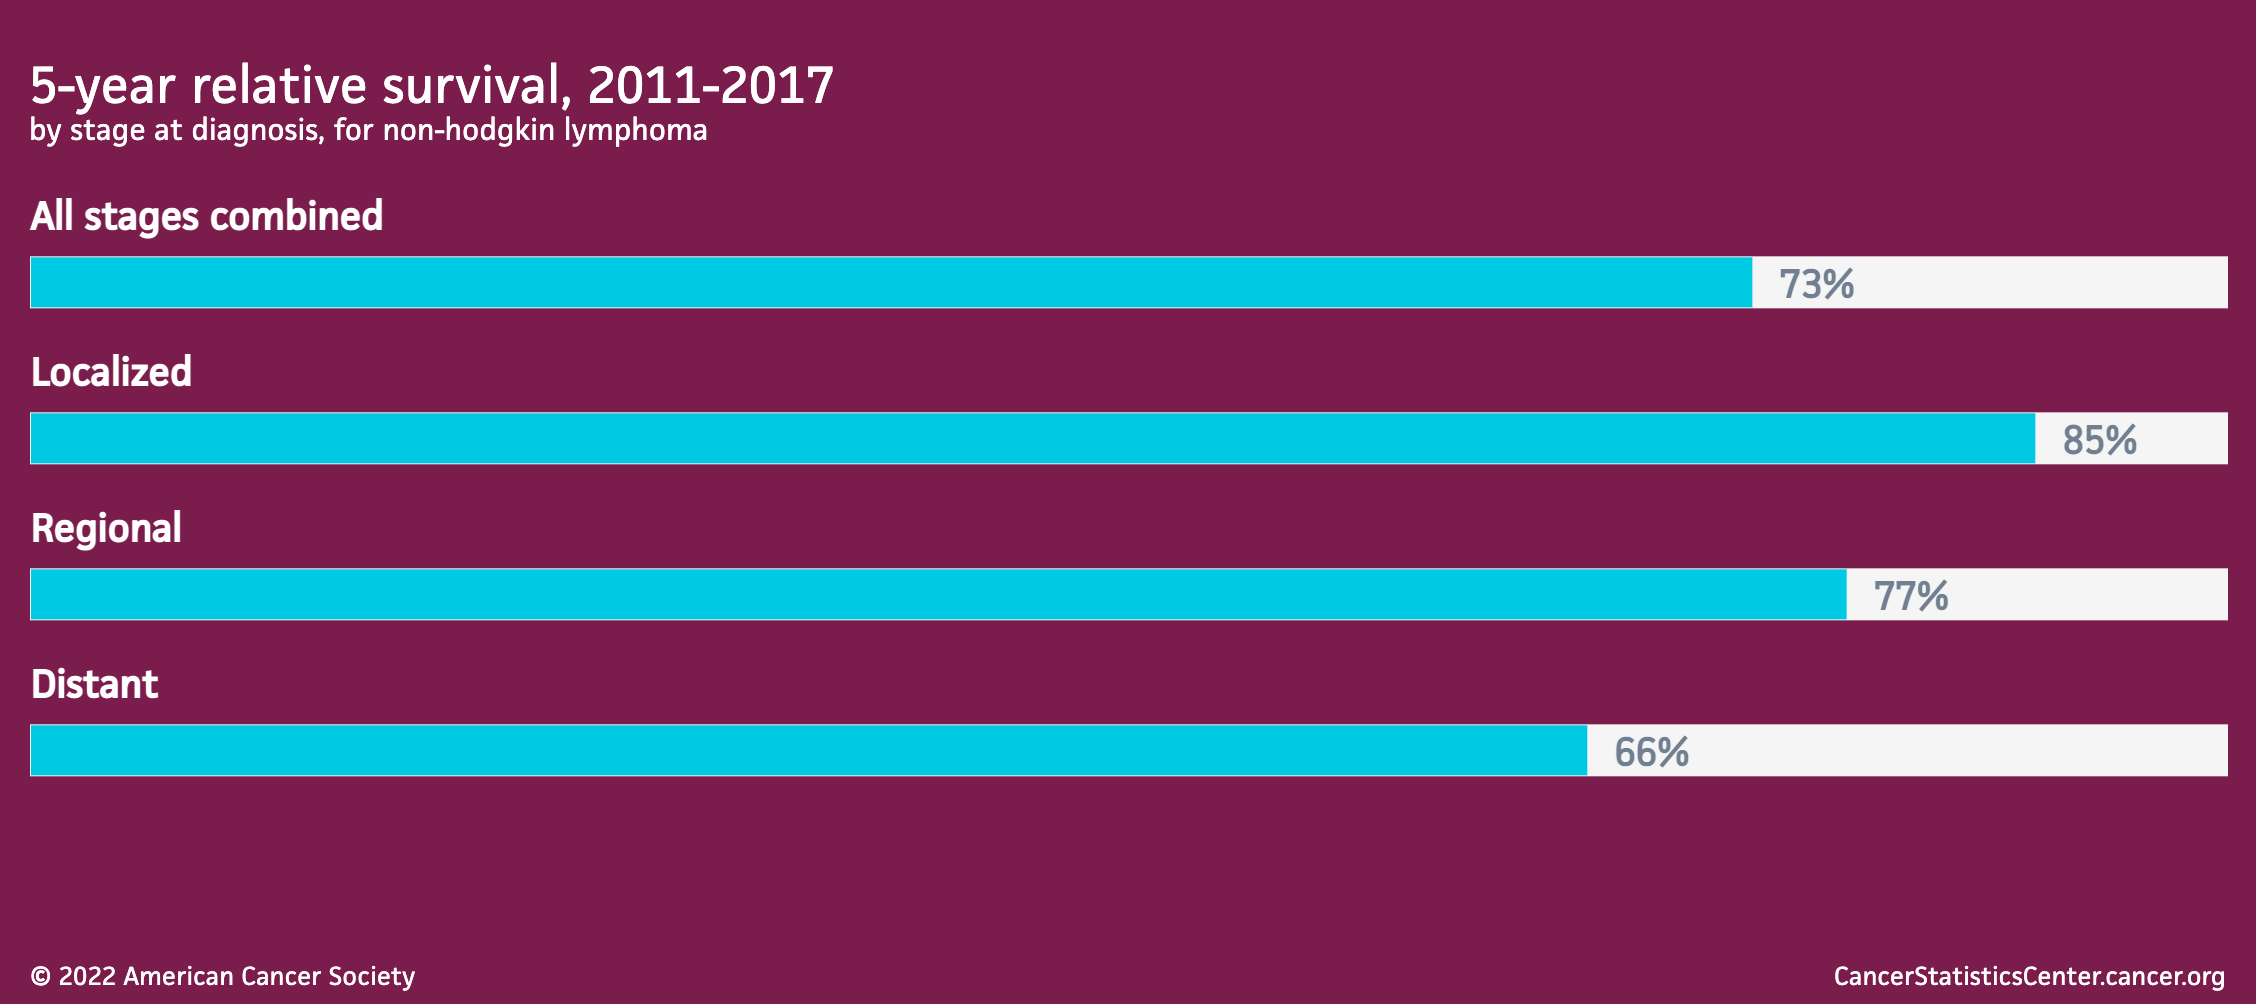
\includegraphics[width=0.7\columnwidth]{img/5-yearrelativesurvival2011-2017.png}
    \end{center}
    \caption[Sopravvivenza a 5 anni, in base allo stato del LNH alla diagnosi, negli Stati Uniti, negli anni 2011-2017]{Sopravvivenza a 5 anni, in base allo stato del LNH alla diagnosi, negli Stati Uniti, negli anni 2011-2017
    \cite{img13}}

\end{figure}

\begin{figure}[H]
    \begin{center}
    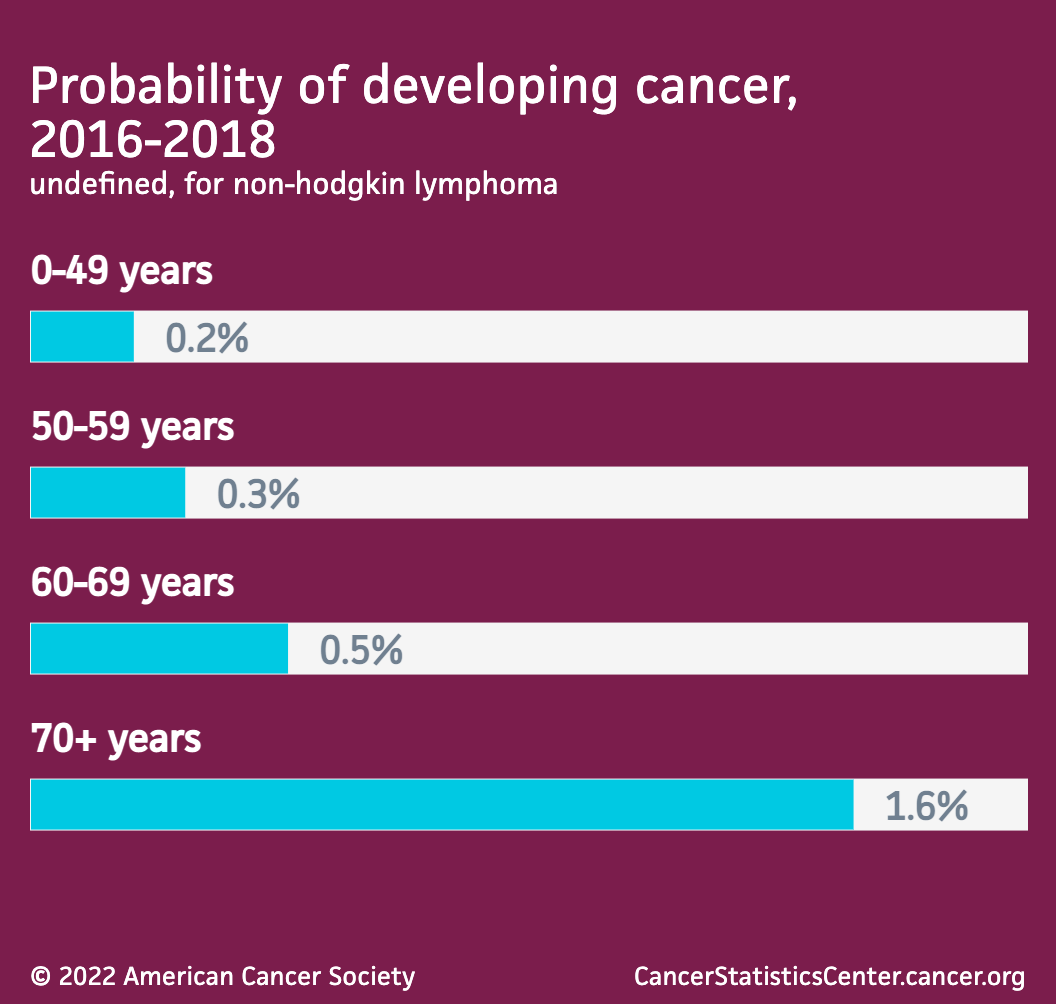
\includegraphics[width=0.4\columnwidth]{img/Probabilityofdevelopingcancer.png}
    \end{center}
    \caption[Probabilità di sviluppare il LNH per fasce d’età, negli Stati Uniti negli anni 2016-2018.]{Probabilità di sviluppare il LNH per fasce d’età, negli Stati Uniti negli anni 2016-2018.
    \cite{img14}}

\end{figure}

\section{Classificazione}
In base alla modalità di crescita e progressione della malattia, i linfomi non-Hodgkin vengono suddivisi in 
linfomi indolenti o a basso grado di malignità, in cui c’è infatti una lenta progressione della malattia, 
non sono presenti sintomi sistemici e le dimensione dei linfonodi affetti aumentano lentamente e tendono a recidivare. 
I linfomi aggressivi o ad alto grado di malignità, sono invece caratterizzati da una rapida progressione della malattia, 
sono associati a sintomi sistemici e necessitano di trattamento tempestivo\cite{reteveneta}.\\

Sono diversi i sottotipi di LNH, attualmente la classificazione segue i criteri proposti dalla WHO 
(World Health Organisation), basati sulla precedente classificazione REAL (Revised European American Lymphoma) 
del 1994 che ha identificato più di 60 tipi di NHL, descritti come unità a sé stanti\cite{AIOM}.\\
La classificazione, identifica i LNH in base alla cellula di origine (linfocita B, T o NK), e quindi si basa su 
criteri morfologici, immunofenotipici, genetici e molecolari, integrati con le caratteristiche di presentazione clinica. 
La classificazione WHO riconosce pertanto tre principali categorie: linfomi a cellule B mature, linfomi a cellule T/NK
mature, linfomi di Hodgkin\cite{AIOM}.\\
Tra i linfomi a cellule B mature, i linfomi diffusi a grandi cellule B (indicati con l’acronimo DLBCL, 
diffuse large B cell lymphoma) sono linfomi aggressivi e da soli rappresentano il sottotipo più frequente, 
sono circa il 25-35\% dei LNH\cite{AIOM}.\\
Il linfoma follicolare (FL) è un linfoma a cellule B e rappresenta circa il 20\% dei NHL.\\

\begin{figure}[H]
    \begin{center}
    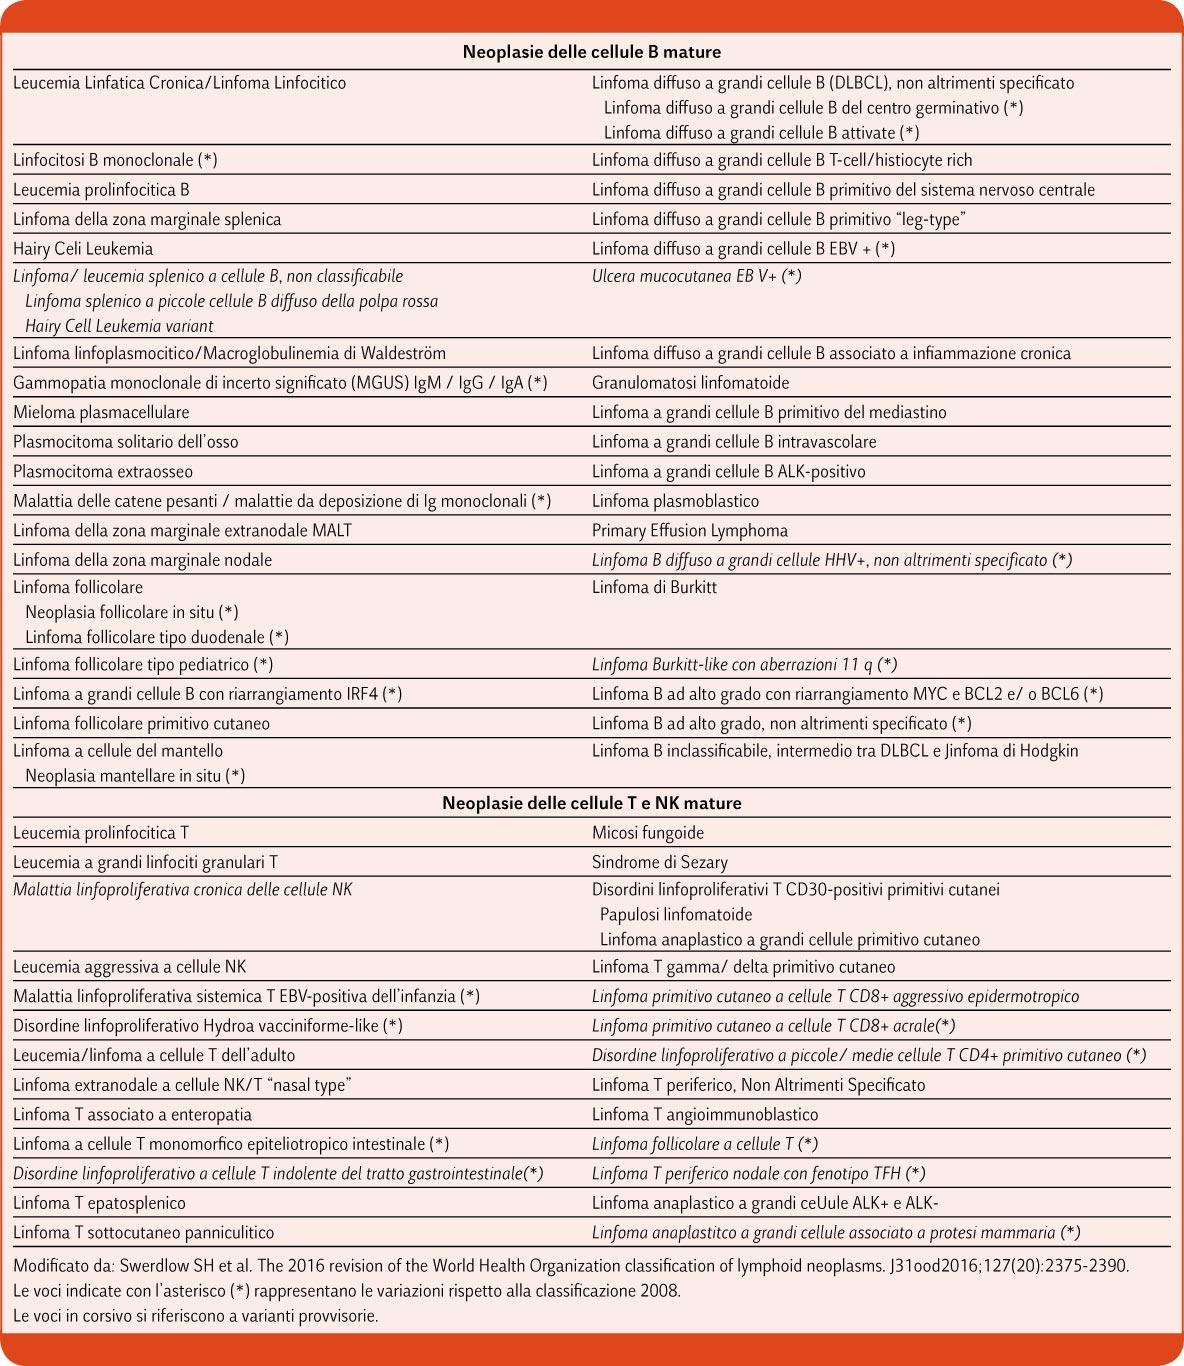
\includegraphics[width=1.0\columnwidth]{img/CLASS.WHO.jpeg}
    \end{center}
    \caption[Classificazione WHO 2016 delle neoplasie linfoidi.]{Classificazione WHO 2016 delle neoplasie linfoidi.
    \cite{img15}}

\end{figure}

\section{Sintomi}
I linfomi, spesso, possono risultare asintomatici e alla diagnosi la malattia si presenta ad uno stadio già avanzato.
Generalmente il sintomo più frequente è l’ingrossamento persistente e non dolente dei linfonodi di ascelle, inguine e 
collo\cite{LNHAIL}.\\ 
Sintomi sistemici invece possono essere febbre, perdita di peso, sudorazione notturna, prurito persistente; 
questi sintomi si manifestano quando sono coinvolti linfonodi profondi, che non possono quindi essere né osservati 
ne palpati e sono più comuni nel caso di linfomi aggressivi.\\ 
I linfomi possono inoltre causare epatomegalia e splenomegalia\cite{AMERICANCANCER}. 
Linfomi più aggressivi, possono colpire organi che non appartengono al sistema linfatico, come stomaco, intestino, 
cute, sistema nervoso, mammella, testicolo, e in tal caso i sintomi sono specifici, cioè dipendono 
dall’organo interessato\cite{AMERICANCANCER}.\\ 
Le cellule tumorali possono anche invadere il sangue, in questo caso si parla di leucemizzazione periferica\cite{LNHAIL}.

\section{Stadiazione}
I linfomi vengono classificati anche in base allo stadio, quindi al grado di estensione della patologia, 
importante al fine di determinare la prognosi e il piano terapeutico più adatto. 
Ad oggi, la stadiazione dei linfomi in quattro stadi, si basa sulla revisione di Lugano che ha sostituito 
la precedente classificazione di Ann-Arbor/Cotswolds\cite{AIOM}.\\
Stadio I, la malattia coinvolge solo una stazione linfonodale, quindi un gruppo ravvicinato di linfonodi. 
Stadio II, la malattia coinvolge due o più stazioni linfonodali, localizzate dallo stesso lato del diaframma. 
Stadio III, la malattia coinvolge stazioni linfonodali su entrambi i lati del diaframma. 
Stadio IV, la malattia coinvolge altri organi, diversi dai linfonodi (ad esempio fegato, polmone o midollo osseo)\cite{LLS}.\\
La lettera B che veniva aggiunta in precedenza se vi erano sintomi sistemici, con la nuova revisione non viene 
più utilizzata, se non per il Linfoma di Hodgkin (LH)\cite{AIOM}.\\
Se il tumore coinvolge un organo esterno al sistema linfatico, come il fegato, si aggiunge la lettera E, 
si aggiunge la lettera S se è coinvolta la milza\cite{ISTGENT}.\\
In caso di massa tumorale con dimensioni voluminose, quindi in caso di condizioni di bulky, 
prima si aggiungeva la lettera X, attualmente non è più necessario, 
bisogna solo dare l’indicazione del diametro maggiore della lesione\cite{AIOM}.\\ 

\begin{figure}[H]
    \begin{center}
    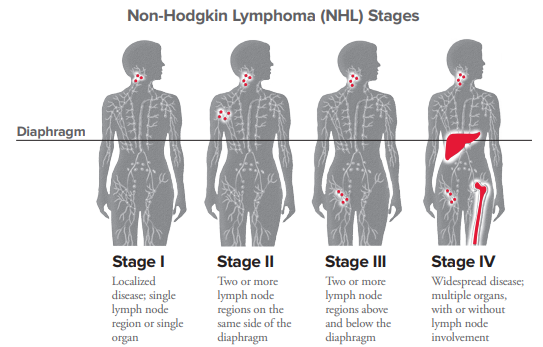
\includegraphics[width=0.85\columnwidth]{img/nhlstages.png}
    \end{center}
    \caption[Stadi del LNH.]{Stadi del LNH.
    \cite{img16}}

\end{figure}

\begin{figure}[H]
    \begin{center}
    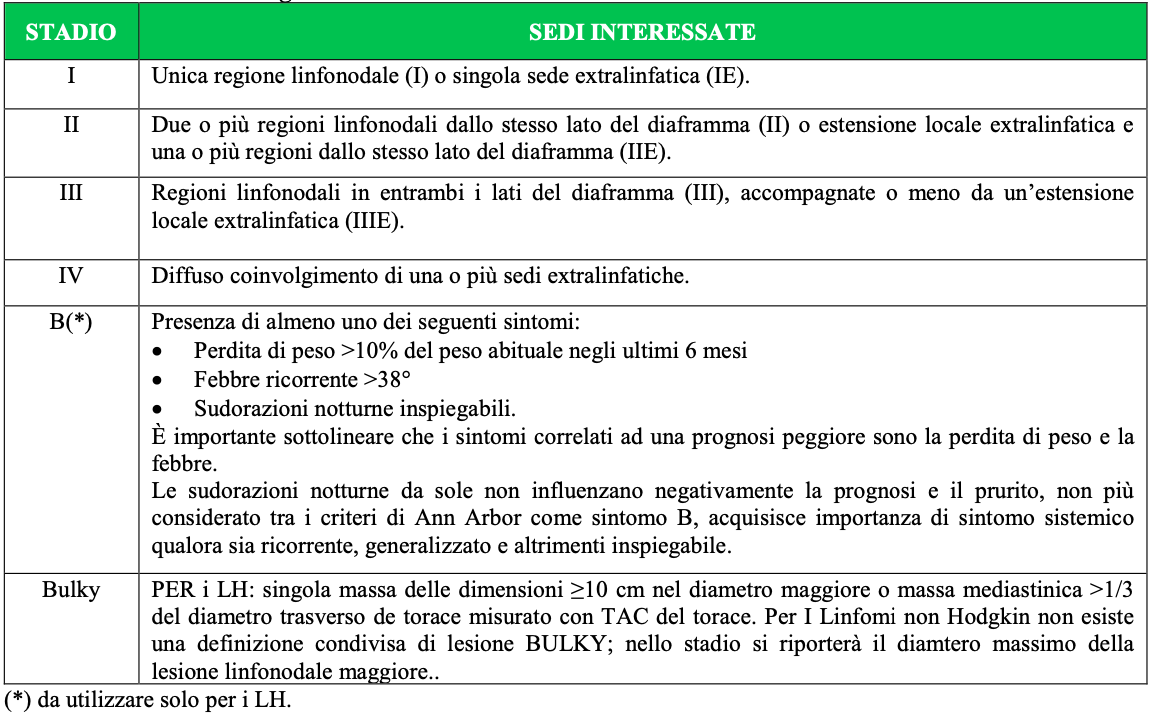
\includegraphics[width=0.95\columnwidth]{img/LUGANOAIOM.png}
    \end{center}
    \caption[Stadi del LNH.]{Stadi del LNH.
    \cite{img17}}

\end{figure}

Per valutare la prognosi dei pazienti con linfoma non-Hodgkin è in uso l’Indice Prognostico Internazionale (IPI). 
Dalla combinazione di una serie di fattori, i pazienti vengono suddivisi in gruppi di rischio: basso, intermedio 
ed alto. 
Per i linfomi diffusi a grandi cellule B (DLBCL) vengono considerati IPI ed aaIPI, cioè IPI “aggiustato per età” 
(age-adjusted IPI)\cite{AIOM}.\\
L’indice prognostico internazionale si basa sulla suddivisione in stadi e prende in considerazione cinque criteri: 
età >60 anni, stadio della malattia (III-IV), malattia presente anche al di fuori del sistema linfatico 
(coinvolgimento di >1 sede extranodale), capacità di svolgere le attività quotidiane >=2 ed elevati livelli 
dell’enzima lattato-deidrogenasi (LDH); elevati livelli ematici di tale enzima indicano la presenza di 
danno tissutale e cellulare. Valori normali sono compresi tra 80 e 300 mU/ml. 
IPI aggiustato per età (aaIPI), è per pazienti con <60 anni, i fattori di rischio per il calcolo sono: 
stadio della malattia (III-IV), performance status >=2, livelli elevati dell’enzima LDH\cite{AIOM}.\\
Attualmente per valutare la prognosi dei pazienti con linfoma follicolare, si utilizza l’indice FLIPI 
(Follicular Lymphoma International Prognostic Index), esso prende in considerazione i seguenti fattori: 
età >60 anni, elevati livelli di LDH sieriche, stadio (III-IV), livelli di Hb inferiori al limite minimo, 
coinvolgimento di >4 sedi linfonodali\cite{AIOM}.\\
Per il linfoma mantellare, l’indice usato è il MIPI (Mantle cell lymphoma International Prognostic Index) e 
i fattori di rischio presi in considerazione in questo caso sono: età, ECOG PS scale 
(Eastern Cooperative Oncology Group Performance Status), livelli di LDH sierici elevati, conta leucocitaria\cite{MIPI}.\\

\begin{figure}[H]
    \begin{center}
    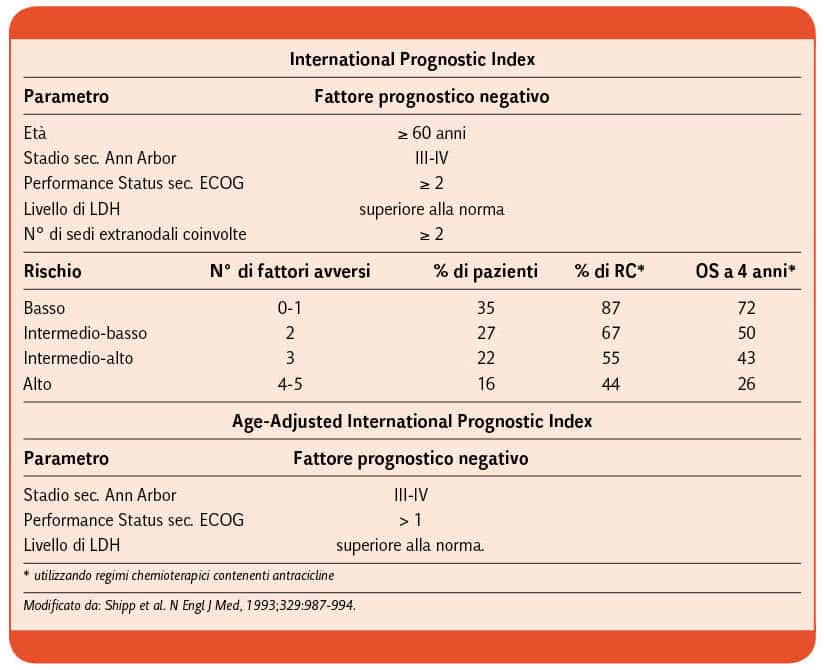
\includegraphics[width=0.8\columnwidth]{img/IPI-AAIPI.jpeg}
    \end{center}
    \caption[IPI ed aaIPI]{IPI ed aaIPI
    \cite{img18}}

\end{figure}

\begin{figure}[H]
    \begin{center}
    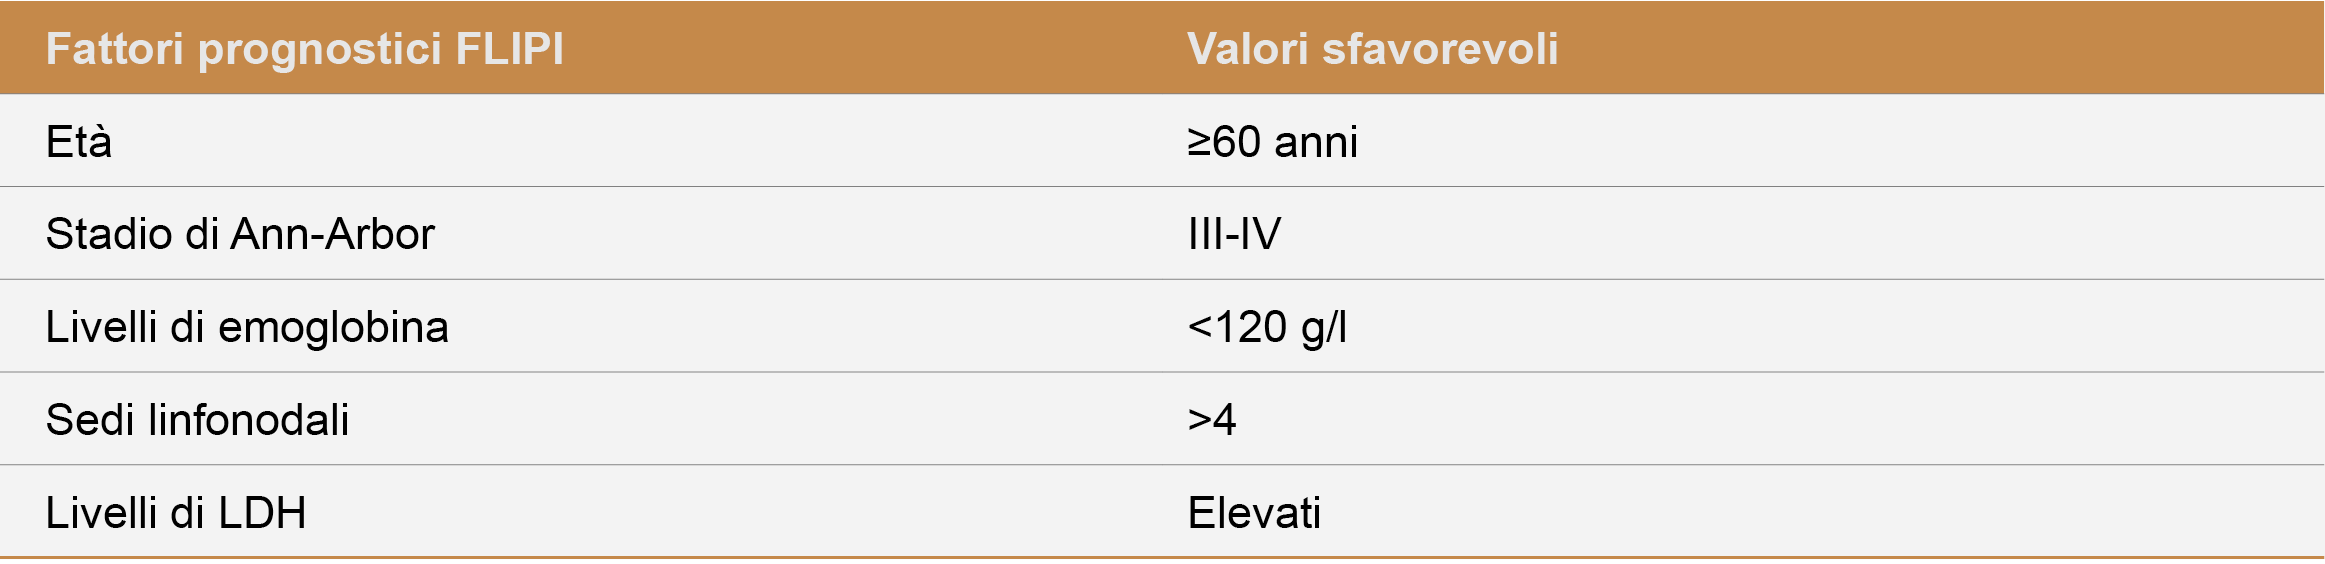
\includegraphics[width=0.8\columnwidth]{img/FLIPI.png}
    \end{center}
    \caption[FLIPI]{FLIPI
    \cite{img19}}

\end{figure}

\begin{figure}[H]
    \begin{center}
    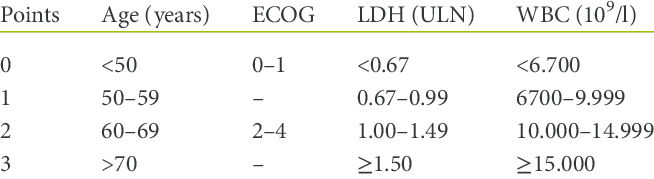
\includegraphics[width=0.8\columnwidth]{img/MIPI.png}
    \end{center}
    \caption[MIPI]{MIPI
    \cite{img20}}

\end{figure}

\section{Diagnosi}
Il gold standard per la diagnosi di linfoma non-hodgkin è la biopsia linfonodale. 
È un esame che consiste nel prelievo di un frammento di tessuto o di un linfonodo, al fine di 
accertarne la loro natura, mediante analisi in laboratorio. 
Generalmente la biopsia viene eseguita in anestesia locale, senza dover ricorrere ad un ricovero; 
se si hanno problemi di accesso al linfonodo, si procede con un intervento in anestesia generale\cite{ISS}.\\
È fortemente raccomandata l’esecuzione di una biopsia escissionale con asportazione dell’intero linfonodo 
oppure una biopsia incisionale, che prevede l’asportazione di un frammento di tessuto\cite{AMERICANCANCER}.\\ 
L’ago aspirato invece è da evitare, in quanto non fornisce un quantitativo di tessuto utile al patologo per formulare 
una diagnosi, si sottopone il paziente ad una procedura non necessaria e si allungano i tempi di formulazione 
della diagnosi\cite{reteveneta}.\\
Un ago-biopsia o core biopsy può essere presa in considerazione come alternativa alla biopsia escissionale/incisionale,
nei casi in cui il linfonodo non risulti accessibile chirurgicamente, in caso di pazienti particolarmente anziani o in 
condizioni di comorbidità; essa è eseguita mediante l’utilizzo di un ago tranciante o ago a scatto, con guida 
ecografica o TC\cite{reteveneta}.\\
Dopo il prelievo, un emolinfopatologo esperto (patologo specializzato nella diagnosi di tali patologie) analizza 
il campione, per verificare la presenza di cellule cancerose, in tal caso viene identificato anche il sottotipo 
istologico o istotipo del linfoma, da cui dipende l’evoluzione del quadro patologico e la scelta del piano 
terapeutico più adatto\cite{LLS}.\\

\section{Esami aggiuntivi a supporto della diagnosi di linfoma non Hodgkin}
Nel momento in cui viene accertata la diagnosi di linfoma di non Hodgkin, si ricorre allo svolgimento di altri 
esami specifici, per analizzare lo stato di salute della persona e l’estensione della malattia.\\
Anamnesi ed esame obiettivo vengono effettuati per la valutazione dei linfonodi superficiali, per quanto riguarda sede, numero, aspetto; 
valutazione di eventuale presenza di epatomegalia o splenomegalia.\\
Si valuta la presenza di sintomi associati come febbre, calo ponderale del peso 
(>10\% negli ultimi 6 mesi senza cause apparenti), sudorazione notturna\cite{reteveneta}.\\
Valutazione del performance status (ECOG) e comorbilità. 
Nel paziente anziano (>65 anni) valutare lo stato di fragilità; in Italia è in uso il modello di 
Valutazione Geriatrica Multidimensionale (VGM), basato sulle scale ADL (valuta le attività di base di vita quotidiana),
 IADL (valuta le attività strumentali di vita quotidiana), CIRS (valuta l’indice di comorbidità), 
 in base al risultato viene stabilita la categoria, fit, unfit, frail\cite{reteveneta}.\\
 Il paziente viene sottoposto ad esami ematochimici per: emocromo, VES, LDH, beta-2 microglobulina, proteine, 
 funzionalità epatica, renale e tiroidea, vitamina D, albumina, test di gravidanza per le donne in età fertile; 
 screening sierologico per HBV, HCV, HIV\cite{AIOM}, \cite{reteveneta}.\\
Effettuare una valutazione dell’attività cardiaca mediante elettrocardiogramma ed ecocardiogramma per valutare 
la frazione di eiezione, nonché una valutazione dell’attività respiratoria mediante spirometria, in vista di 
trattamenti con farmaci che potrebbero avere degli effetti su di esse\cite{AIOM}.\\ 
Per i pazienti in età fertile che si sottoporranno a chemioterapia sterilizzante, prevedere un programma di 
criopreservazione del liquido seminale per l’uomo e degli ovociti per la donna, valutando l’eventuale assunzione di 
estroprogestinico, LH-RH o analoghi\cite{AIOM}.\\
La diagnostica per immagini può prevedere la TC collo, torace e addome o pelvi con mdc; la radiografia del torace 
in due proiezioni associato all’ecografia dell’addome completo, possono sostituire la TC in caso di pazienti 
anziani con disordini linfoproliferativi a decorso indolente.
La PET-TC total body con 18 FDG (Fluorodesossiglucosio) è raccomandata nei linfomi detti “PET avidi” come il DLBCL, 
linfoma follicolare, mantellare, linfomi a cellule T; essa è inoltre indicata nel caso di linfomi indolenti con 
sospetta trasformazione istologica. Nei pazienti con malattia non avida per FDG si può optare per la TC\cite{reteveneta}.\\ 
Nei pazienti con malattia avida, la risposta alla PET viene valutata mediante i criteri di Deauville. 
La risposta al trattamento può essere di remissione completa (RC) con punteggio Deauville 1-3, si ha 
la scomparsa della malattia in ogni sede e dei sintomi ad essa correlati, rientrano nella categoria RC pazienti 
con PET positiva che ottengono una PET negativa; remissione parziale (RP), punteggio Deauville 4-5, riduzione 
delle adenopatie superiore al 50\%, senza comparsa di nuove lesioni, la PET può essere positiva sulle sedi iniziali 
di malattia non incrementate; malattia stabile (MS), punteggio Deauville 4-5, PET positiva sulle sedi iniziali di 
malattia senza comparsa di nuove lesioni; progressione (PG), punteggio Deauville 5, comparsa di nuove lesioni 
alla PET e aumento superiore al 50\% delle dimensioni delle lesioni linfomatose presenti all’inizio del trattamento\cite{AIOM}.\\

\begin{figure}[H]
    \begin{center}
    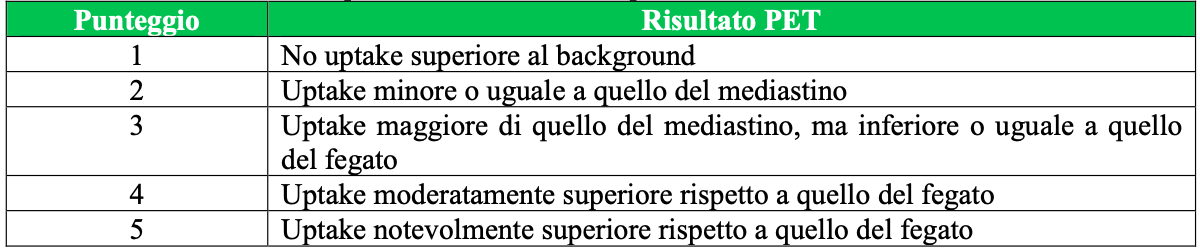
\includegraphics[width=0.9\columnwidth]{img/DEAUVILLE.png}
    \end{center}
    \caption[Criteri di Deauville per la valutazione della risposta alla PET.]{Criteri di Deauville per la valutazione della risposta alla PET.
    \cite{img21}}

\end{figure}

In casi specifici, si valuta la necessità di ricorrere a:\\ 
- Biopsia osteo-midollare (BOM), è eseguita per prelevare un frammento di tessuto dalla cresta iliaca posteriore 
superiore, per accertarsi che la malattia non si sia diffusa al midollo spinale; se il paziente ha una PET positiva 
su osso, questa procedura può non essere eseguita.\\
- Visita otorinolaringoiatrica, nel caso in cui si sospetti o si sia accertata una localizzazione rino-oro-faringea.\\
- TC/RMN cerebrale, scintigrafia scheletrica, ecografia testicolare, rx o endoscopia del tratto gastroenterico, 
da eseguire in caso di localizzazione dubbia o sospetta a livello del SNC.\\
- Esame citologico chimico-fisico del liquido cefalo-rachidiano, in caso di rischio di diffusione meningea, 
mediante puntura lombare o rachicentesi\cite{AIOM}.\\






